\documentclass[11pt, journal, onecolumn, letterpaper,]{LaTeX_Assets/IEEETransactions_LaTeX/IEEEtran/IEEEtran}
\usepackage{graphicx}
\graphicspath{{./jpeg/}{LaTeX_Assets/jpeg/}}
\usepackage{float}
\usepackage{bytefield}
\usepackage{tikz}
\usetikzlibrary{automata, positioning, arrows, calc}
\tikzset{
->, % makes the edges directed
>=stealth', % makes the arrow heads bold
node distance=4cm, % specifies the minimum distance between two nodes. Change if necessary.
every state/.style={thick, fill=gray!10}, % sets the properties for each 'state' node
initial text=$ $, % sets the text that appears on the start arrow
}
\usepackage{caption}
\captionsetup[table]{skip=10pt}

\begin{document}

    \title{Routing Implementation Considering Proactive Effective Redundant Routes, Infrastructureless (RIC-PERRI)}
    \author{Stephen~Donchez,~\IEEEmembership{Member,~IEEE}%
    \thanks{S. Donchez is with Villanova University, Villanova, PA 19085 USA 
    \mbox{(e-mail:sdonchez@villanova.edu)}}%
    \thanks{Manuscript received May 4, 2022}}%

    \maketitle

    % %!TeX root = ../ECE8408_Project_Ad_Hoc_Routing.tex
\section*{Abstract}
Mobile Ad-Hoc Networks (MANETs) require the implementation of non-conventional routing protocols to accommodate their nature as an infrastructureless network that functions using peer-based multi-hop routing. These networks have been deployed with increasing frequency in recent years for a variety of use cases, including disaster response. This paper proposes a routing algorithm, RIC-PERRI, which seeks to address the unique needs of routing in such a critical response scenario, where highly reliable communications links are essential and node disconnections could have life or death consequences. The algorithm addresses these needs by precomputing redundant routes for all nodes in a system, as well as enabling proactive notifications for any detected instances of node failure. The algorithm is derived from the ubiquitous Distance Vector routing protocol, and takes strides where possible to ensure compatibility with the packet formats and conventions utilized by it and many similar protocols to ease implementation and adoption.

    %!TeX root = ../ECE8408_Project_Ad_Hoc_Routing.tex
\section{Introduction}\label{sec:introduction}
\IEEEPARstart{M}{obile} Ad-Hoc Networks, or MANETs, are a subset of network communication systems that operate in an Infrastructure-less environment. These networks are well suited to a number of fairly niche use cases, including incident response and disaster recovery, third-world and underdeveloped areas, and for military applications. By virtue of their application, as well as their infrastructure-less nature, these networks require extensive peer-to-peer communications, including peer-based routing. Such a routing algorithm necessarily differs from the conventional Open Shortest Path First (OSPF) and Distance Vector (DV) based algorithms such as are implemented in conventional networks.

\subsection{Routing Algorithm Objectives}\label{subsec:objectives}

This paper proposes a \textbf{R}outing \textbf{I}mplementation \textbf{C}onsidering \textbf{P}roactive \textbf{R}edundant \textbf{R}outes for \textbf{I}nfrastructureless systems, or \textbf{RIC-PERRI} \cite{perry_rp_2022} for short. The algorithm is intended for critical responders in emergency situations, where reliable connections can quite literally be a life-or-death concern. To this end, the algorithm is based on a proactive routing scheme, wherein routes for all nodes are calculated up front, and a full refresh is performed periodically. This is critical, as a node becoming disconnected could indicate a responder in grave danger, and being unaware of this until some random node needs to send a message to the node in question is unacceptable under these circumstances. To the same end, the algorithm computes both a primary and a secondary route for each node, such that a compromised link does not require a routing data update prior to attempting a retransmission of the message in question. 

In order to ensure reliable transmission of data, the routing algorithm considers Received Signal Strength Indicator (RSSI) values as a factor in computing routes. RSSI is defined in IEEE Standard 802.11 as ``a measure by the PHY of the energy observed at the antenna connector used to receive the current PPDU [Physical Layer Protocol Data Unit]''\cite{lanman_standards_committee_80211-2020_2021}. It should be noted that RSSI is measured by the receiver, as opposed to the majority of routing information, which is provided by the originator of routing data.

Although a reliable connection is crucial to the transmission of data, there is not necessarily any benefit to be gained from one sufficiently reliable connection over another, even if the former is of appreciably higher RSSI than the latter. That is, any link that possess an RSSI over a given threshold is equally suited to the transmission of data. Accordingly, this algorithm will not seek to utilize RSSI as a metric in the route selection process, but rather as a a prerequisite for a link being valid as an option for consideration. The RSSI value threshold for such a decision is parameterized and left to the implementer, but it is suggested that such a value be sufficiently high that it allow for all but guaranteed delivery of data.

Instead, the algorithm shall employ an adapted Distance Vector based approach that is optimized to minimize hop count on all routes. This method was chosen for several reasons. First and foremost, the implementation of a DV-based protocol ensures a lightweight and non resource-intensive routing scheme, especially as compared to a more complex OSPF-based algorithm. Furthermore, MANETs deployed to support critical responders are likely to be fairly compact, meaning that there will likely be low propagation delays relative to the queuing delays within each device. Therefore, minimizing hops will reduce the number of queuing delays encountered, ensuring efficient delivery.

The chief modifications this algorithm proposes to Distance Vector relate to the increased need for constant communication in a critical response environment. The protocol adopts the concept of sequenced routing updates from the Destination-Sequenced Distance Vector (DSDV) protocol, originally proposed in \cite{perkins_highly_1994}. As was previously mentioned, each node also maintains two routes for each destination, ensuring redundancy provided the routes do not share common links. Given that a critical response situation is likely small and concentrated, such a network approximates a full-mesh network, making this likely. Finally, the system implements node failure notifications that are broadcast to all nodes upon detection of an inability to reach a given node, which can be used to trigger application-layer responses such as audible alarms, etc.

\subsection{Organization of this Work}\label{subsec:IntroOrganization}
The remainder of this work is organized into five primary sections. Section \ref{sec:stateMachine} provides a functional specification of the algorithm by means of a Finite State Machine (FSM) and accompanying comments. Section \ref{sec:packetDefinitions} defines the various fields and structures used in the packets sent by this algorithm. Section \ref{sec:informalProof} provides a set of informal proofs to demonstrate the correctness of the algorithm under various conditions and failure modes. Finally, \ref{sec:conclusion} concludes the work with a brief summary of the algorithm, as well as a discussion of avenues for its enhancement in the future.

    %!TeX root = ../ECE8408_Project_Ad_Hoc_Routing.tex
\section{Algorithm State Machine}\label{sec:stateMachine}
\subsection{Final State Machine}\label{subsec:SMfinalStateMachine}
The various steps in the RIC-PERRI Routing algorithm can be captured in a Finite State Machine (FSM), as shown in Figure \ref{fig:finalStateMachine}. For purposes of brevity, the FSM uses numerical IDs for each state. Descriptions of each state are presented in Table \ref{table:FSMDescriptions}. State transitions without labels represent unconditional or default transitions.

\begin{figure}[ht]
    \centering
    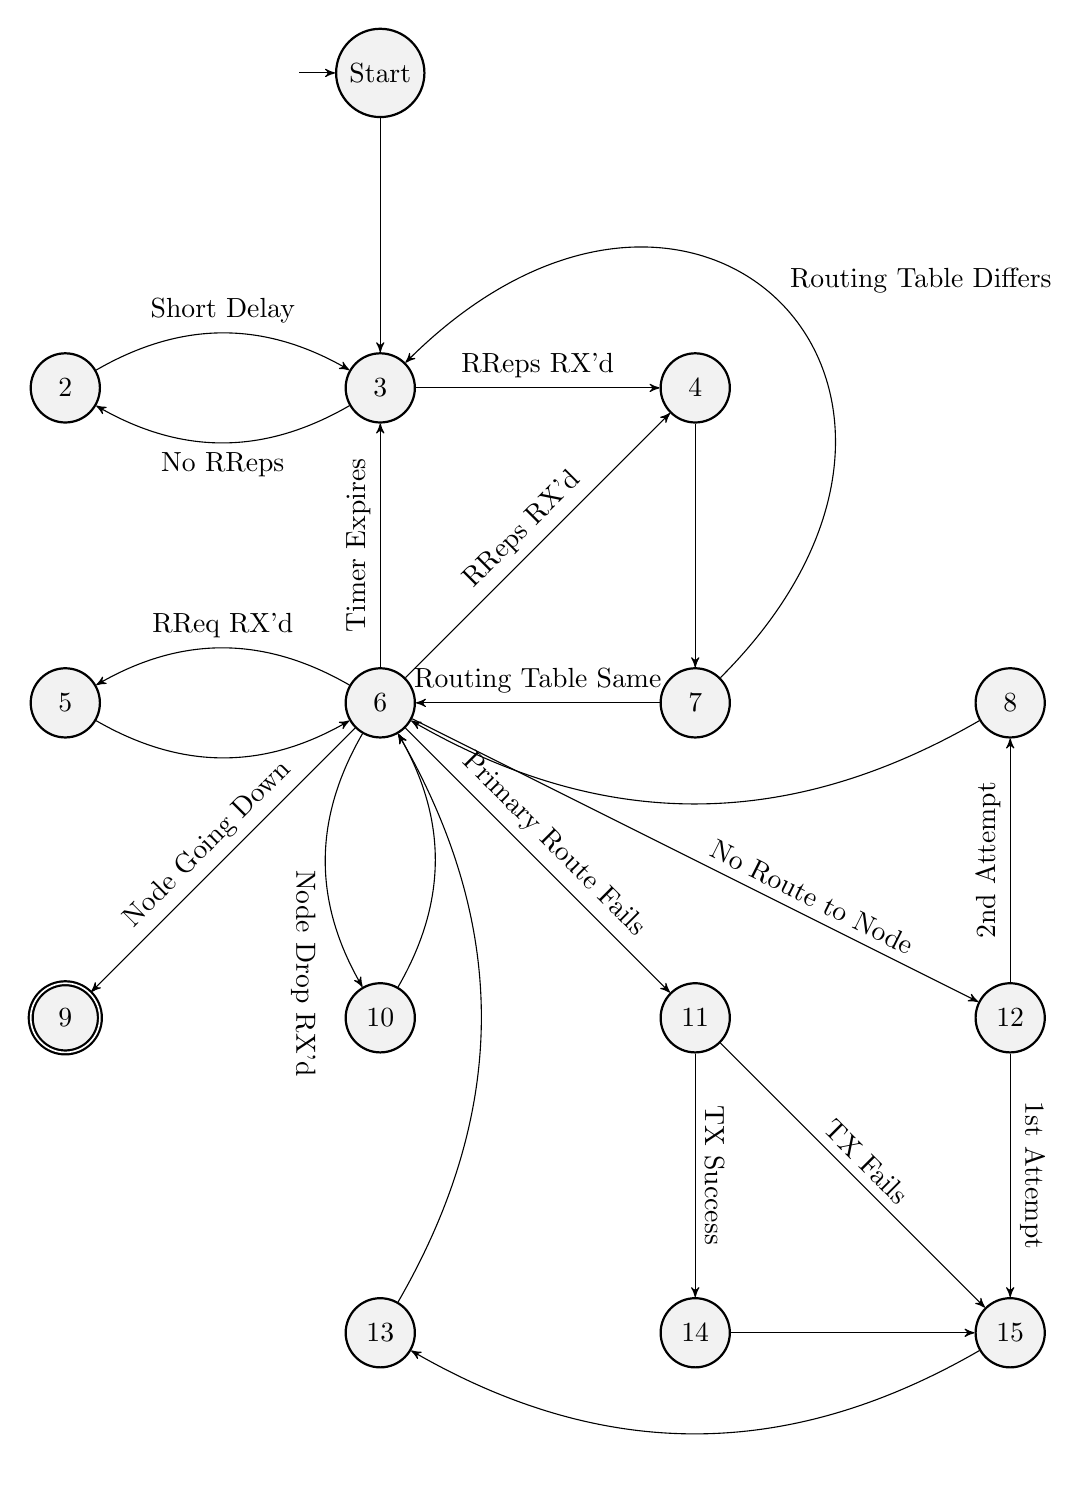
\begin{tikzpicture}
        \node[state,initial](q1) {Start};
        \node[state, below of=q1] (q3) {3};
        \node[state, left of=q3] (q2) {2};
        \node[state, right of=q3] (q4) {4};
        \node[state, below of=q2] (q5) {5};
        \node[state, below of=q3] (q6) {6};
        \node[state, below of=q4] (q7) {7};
        \node[state, right of=q7] (q8) {8};
        \node[state, below of=q5, accepting] (q9) {9};
        \node[state, right of=q9] (q10) {10};
        \node[state, right of=q10] (q11) {11};
        \node[state, right of=q11] (q12) {12};
        \node[state, below of=q10] (q13) {13};
        \node[state, right of=q13] (q14) {14};
        \node[state, right of=q14] (q15) {15};
        % \node[state, right of=q9] (q14) {14};
        % \node[state, left of=q9] (q15) {15};

        \draw (q1) edge [above] node {} (q3)
            (q2) edge [bend left, above] node {Short Delay} (q3)
            (q3) edge [bend left, below] node {No RReps} (q2)
            (q3) edge [above] node {RReps RX'd} (q4)
            (q4) edge [above] node {} (q7)
            (q5) edge [bend right] node {} (q6)
            (q6) edge [sloped, anchor=center, above] node {Timer Expires} (q3)
            (q6) edge [sloped, anchor=center, above] node {RReps RX'd} (q4)
            (q6) edge [above, bend right] node {RReq RX'd} (q5)
            (q6) edge [sloped, anchor=center, above] node {Node Going Down} (q9)
            (q6) edge [sloped, anchor=center, below right, bend right] node {Node Drop RX'd} (q10)
            (q6) edge [sloped, anchor=center, above] node {Primary Route Fails} (q11)
            (q6) edge [sloped, anchor=center, above right] node {No Route to Node} (q12)
            (q7) edge [above] node {Routing Table Same} (q6)
            (q8) edge [above, bend left] node {} (q6)
            (q10) edge [bend right] node {} (q6)
            (q11) edge [sloped, anchor=center, above] node {TX Success} (q14)
            (q11) edge [sloped, anchor=center, above] node {TX Fails} (q15)
            (q12) edge [sloped, anchor=center, above] node {2nd Attempt} (q8)
            (q12) edge [sloped, anchor=center, above] node {1st Attempt} (q15)
            (q13) edge [bend right] node {} (q6)
            (q14) edge [] node {} (q15)
            (q15) edge [below, bend left] node {} (q13)
            ;
            \draw [->] (q7) ..  controls  ($(q7)+(4cm,4cm)$) and
  ($(q3)+(4cm,4cm)$) ..  (q3) node[midway,above right] {Routing Table Differs};
    \end{tikzpicture}
    \caption{RIC-PERRI Algorithm State Machine}
    \label{fig:finalStateMachine}
\end{figure}
\begin{table}[ht]
    \centering\begin{tabular}{|c|c|}
        \hline
        State ID & Description \\
        \hline
        \hline
        1 & Initial State \\
        \hline
        2 & Notify user of isolation, enter brief delay \\
        \hline
        3 & Broadcast RReq for all routes \\
        \hline
        4 & Receive Full Routing Data \\
        \hline
        5 & Transmit any known requested routes \\
        \hline
        6 & Set timer and wait for expiration \\
        \hline
        7 & Generate Full Routing Table \\
        \hline
        8 & Transmit Node Drop Alert, Remove Routes to Node\\
        \hline
        9 & Alert all other nodes, advertise all known routes at infinite cost \\
        \hline
        10 & Remove Routes to Node, alert user (layer 7) \\
        \hline
        11 & Transmit message over secondary route \\
        \hline
        12 & Alert user of unreachable node \\
        \hline
        13 & Perform partial routing table update \\
        \hline
        14 & Promote secondary route to primary \\
        \hline
        15 & Send specific RReq \\
        \hline

    \end{tabular}
    \caption{Failure Notification Statuses}
    \label{table:FSMDescriptions}
\end{table}

As can be seen in the state machine diagram, the ``normal'' operation of the algorithm is fairly straight forward, and in keeping with traditional DV-based implementations. Upon initialization (the ``Start'' State), the algorithm transmits a Route Request (RReq) for all nodes in the network (State 3). It then collects Route Responses (RRes) from its neighbors (State 4), and constructs a routing table (State 7) containing dual routes for each node. It repeats this process until the table is constant for two iterations, at which point it assumes it has found all routes. It then enters a delay state (State 6), wherein it sets a timer for a parameter-defined time, and waits for said timer to expire before repeating the process.

The other ``normal'' operations a node performs are related to responding to routing requests and responses. The former, captured in State 5 of the FSM, requires the node to transmit select routes in response to a query, or all routes if select routes are not specified.  After completing this requirement, the algorithm transitions back to its normal state of waiting for the timer to expire. Meanwhile, the latter is captured in the State 6 $\rightarrow$ State 4 transition, where the node receives an un-requested response (due to another node updating its routes). The node updates its routes based on this information, goes through the routing update process to ensure that other changes don't result, and then resumes normal operation.

The simplest failure case in this algorithm (but also the most severe) is captured in State 2. This state represented the case where the node, upon performing a request for all routes, receives no responses. This indicates that the node has become isolated from the network. While this is obviously a dire state (especially given the intended use case), there is very little that can be done beyond alerting the user. After doing so, the node waits a brief period of time before re-transmitting the request. 

Similarly, State 9 in the diagram represents the case where a node is intentionally dropping from the network, either due to being powered down (at the completion of operations) or due to depleted battery, etc. In this case, the node proceeds to alert all other nodes that it is going down, which triggers them to update routes with that node listed as a next hop to a cost of $\infty$ and send out unsolicited route responses. Depending on the nature of the disconnection, other nodes can then provide a user alert if necessary. 

The lower right portion of the FSM diagram in Figure \ref{fig:finalStateMachine} represents the more complex failure states. The link from State 6 to State 12 represents the case where a route is requested to a node which does not have a routing table entry, either due to it having been removed or due to it being a node that has never previously been recognized by the current node. In this case, the node will attempt to perform a specific Route Request for the target node (State 12 $\rightarrow$ 15 $\rightarrow$ 13). If this fails, it will perform a second attempt before giving up and notifying the user (State 8).

Meanwhile, State 11 handles the case where a where a node is unable to transmit along a known route. If this is the case, the node immediately attempts to utilize the secondary route that was pre-computed. If this is successful, it promotes that to the primary route temporarily (State 14). Regardless of success, it transmits a selective RReq for that node in an attempt to restore the redundancy of the connection (State 15), and updates the table based on the responses (State 13).

\subsection{Iterative Improvements}\label{subsec:SMiterativeImprovements}
The Finite State Machine proposed above underwent a number of revisions aimed at improving its performance, as well as addressing edge cases which were not previously considered. For example, the handling of a node that is advertising its own imminent disconnection was greatly enhanced. In the original design, the node sent out a notification that it was going down, which would be used by other nodes with it in their routing tables to seek new routes. However, the nature of a DV-based algorithm is such that it is not immediately obvious what nodes depend on a given link, as each node only retains its "next hop" information. To rectify this, the algorithm was modified so that each adjacent node, upon updating its tables, would send an unsolicited RRep packet, with a cost of $\infty$ for the node that is disconnecting. This allows other nodes to update their tables, after which they would issue similar packets, and the process would continue. This required a new transition in the state machine, specifically the one from State 6 $\rightarrow$ State 4.
    %!TeX root = ../ECE8408_Project_Ad_Hoc_Routing.tex
\section{Packet Definitions}\label{sec:packetDefinitions}
The RIC-PERRI algorithm utilizes the common Internet Group Message Protocol (IGMP) packet format utilized by the traditional Distance Vector Multicast Routing Protocol (DVMRP, or just DV) algorithm upon which it is based. Many of the fields below are adopted directly from the RFC which proposes the DVMRP protocol, RFC 1075 \cite{waitzman_distance_1988}. The subsections below begin by describing the individual fields that can be used to construct the various packets, followed by the various packets themselves.
\subsection{Available Fields}\label{subsec:PDAvailableFields}
The following fields are used to construct the packets needed by the RIC-PERRI protocol. Where noted, these fields are directly adopted from \cite{waitzman_distance_1988}. In the literature, these fields are sometimes referred to as \emph{commands}. This work uses these terms interchangeably.

\subsubsection{IGMP Header}\label{subsubsec:PDAFIGMPHeader}
The IGMP header is common to all packets in the algorithm. Each individual packet type is indicated by a subtype in the appropriate field, as defined in Figure \ref{fig:IGMPHeader}. This field is directly adopted from \cite{waitzman_distance_1988}.
\begin{figure}[H]
    \centering
    \begin{bytefield}[bitwidth=1.4em]{32}
        \bitheader{0-31}\\
        \bitbox{4}{Version=1} & \bitbox{4}{Type=8} & \bitbox{8}{Subtype} & \bitbox{16}{Checksum}
    \end{bytefield}
    \caption{IGMP Header Specification}
    \label{fig:IGMPHeader}
\end{figure}
The IGMP Header, adopted from \cite{waitzman_distance_1988}, identifies the packet as an Internet Group Management Protocol (IGMP) packet. The version field is set to 1, indicating that the packet is an IGMP version 1 datagram. The type field is set to 8, which is not otherwise utilized according to IANA \cite{fenner_iana_2002}. This will serve as the identifier for RIC-PERRI messages. The subtype field is used to indicate the type of packet being sent, as indicated in Table \ref{table:IGMPHeaderSubtypes}, below:
\begin{table}[H]
    \centering\begin{tabular}{|c|c|}
        \hline
        Subtype ID & Subtype \\
        \hline
        \hline
        1 & Routing Update \\
        \hline
        2 & Routing Query \\
        \hline
        3 & Dropped Node \\
        \hline
        4 - 255 & Reserved \\
        \hline
    \end{tabular}
    \caption{IGMP Header Subtypes}
    \label{table:IGMPHeaderSubtypes}
\end{table}

\subsubsection{Metric Value}\label{subsubsec:PDAFMetricValue}
The metric value, used messages providing route details, provides the ``cost'' value associated with a given address. The metric is has a maximum value of 255, and is further constrained by the Infinity Value, as outlined in Field \ref{subsubsec:PDAFInfinityValue}, below. This field is directly adopted from \cite{waitzman_distance_1988}.
\begin{figure}[H]
    \centering
    \begin{bytefield}[bitwidth=1.4em]{16}
        \bitheader{0-15}\\
        \bitbox{8}{Command=4} & \bitbox{8}{Value}
    \end{bytefield}
    \caption{Metric Command Specification}
    \label{fig:MetricCommand}
\end{figure}

\subsubsection{Infinity Value}\label{subsubsec:PDAFInfinityValue}
The infinity command is used to indicate the minimum value of the metric which is considered to be an infinite cost. Any value greater than or equal to this value is considered to be infinite, meaning that a route with a cost at or above this value will not be considered a valid option. This field is directly adopted from \cite{waitzman_distance_1988}.
\begin{figure}[H]
    \centering
    \begin{bytefield}[bitwidth=1.4em]{16}
        \bitheader{0-15}\\
        \bitbox{8}{Command=6} & \bitbox{8}{Value}
    \end{bytefield}
    \caption{Infinity Command Specification}
    \label{fig:InfinityCommand}
\end{figure}

\subsubsection{Destination Address Command}\label{subsubsec:PDAFDestinationAddressCommand}
The destination address command is used to indicate available routes. It is used in the routing update process, and contains a given number of destinations, as specified by the count value. Each destination is represented by a 32-bit IP Address, followed by another 32-bit IP Address indicating the next hop to be followed. Destinations are always presented as a pair of 32 bit fields, a destination and a next hop. Subsequent pairs follow the same format. Each message has an incremental sequence number to prevent stale routes. This sequence number is specific to the sender, not common across the network. This field is adopted from \cite{waitzman_distance_1988}, with some modification. Specifically, the concept of a sequence number to ensure that stale routes are not persisted is adopted from the Destination-Sequenced Distance Vector protocol, proposed in \cite{perkins_highly_1994}.
\begin{figure}[H]
    \centering
    \begin{bytefield}[bitwidth=1.1em]{32}
        \bitheader{0-31}\\
        \bitbox{8}{Command=7} & \bitbox{8}{Count=$N$} & \bitbox{16}{Sequence Number} \\
        \begin{rightwordgroup}{Route 1}
            \bitbox{32}{Destination} \\
            \bitbox{32}{Next Hop}
        \end{rightwordgroup} \\
        \begin{rightwordgroup}{Route 2}
            \bitbox{32}{Destination} \\
            \bitbox{32}{Next Hop}
        \end{rightwordgroup} \\
        \wordbox[]{1}{$\vdots$} \\[1ex]
        \begin{rightwordgroup}{Route $N$}
            \bitbox{32}{Destination} \\
            \bitbox{32}{Next Hop}
        \end{rightwordgroup}
    \end{bytefield}
    \caption{Destination Address Command Specification}
    \label{fig:DestinationAddressCommand}
\end{figure}

\subsubsection{Request Destination Address (RDA) Command}\label{subsubsec:PDAFRequestedDestinationAddressCommand}
The requested destination address command is used to request available routes. It is used in the routing update process, and contains a given number of requested destinations, as specified by the count value. Alternatively, the count value can be set to zero, requesting all available routes. Each destination is represented by a 32-bit IP Address. This field is adopted from \cite{waitzman_distance_1988}, with some modifications.
\begin{figure}[H]
    \centering
    \begin{bytefield}[bitwidth=1.1em]{32}
        \bitheader{0-31}\\
        \bitbox{8}{Command=8} & \bitbox{8}{Count=$N$} & \bitbox{16}{Reserved} \\
        \begin{rightwordgroup}{Destination 1}
            \bitbox{32}{Requested Destination}
        \end{rightwordgroup} \\
        \begin{rightwordgroup}{Destination 2}
            \bitbox{32}{Requested Destination}
        \end{rightwordgroup} \\
        \wordbox[]{1}{$\vdots$} \\[1ex]
        \begin{rightwordgroup}{Destination $N$}
            \bitbox{32}{Requested Destination}
        \end{rightwordgroup}
    \end{bytefield}
    \caption{Requested Destination Address Command Specification}
    \label{fig:RequestedDestinationAddressCommand}
\end{figure}

\subsubsection{Failure Notification}\label{subsubsec:PDAFFailureNotification}
The failure notification is used to indicate some form of failure in the routing process. This can include a failure to transmit a packet over a known route, or the inability to find a route to a given node.
\begin{figure}[H]
    \centering
    \begin{bytefield}[bitwidth=1.1em]{32}
        \bitheader{0-31}\\
        \bitbox{8}{Command=F} & \bitbox{8}{Status} & \bitbox{16}{Reserved} \\
        \bitbox{32}{Address}\\
    \end{bytefield}
    \caption{Failure Notification Specification}
    \label{fig:FailureNotification}
\end{figure}
\begin{table}[H]
    \centering\begin{tabular}{|c|c|}
        \hline
        Status ID & Status \\
        \hline
        \hline
        1 & Node Unreachable \\
        \hline
        2 & Node Intentional Disconnect \\
        \hline
        3 & Node Unintentional Disconnect \\
        \hline
        4 - 255 & Reserved \\
        \hline
    \end{tabular}
    \caption{Failure Notification Statuses}
    \label{table:FailureNotificationStatuses}
\end{table}
\subsection{Packet Formats}\label{subsec:PDpacketFormats}
    %!TeX root = ../ECE8408_Project_Ad_Hoc_Routing.tex
\section{Informal Proof}\label{sec:informalProof}
Although this routing protocol is (at this time) solely theoretical in nature, efforts have been undertaken to ensure its functionality and efficiency in a representative environment, with special attention to its handling of unusual circumstances. The various below subsections address these concerns, outlining a brief informal proof of the function of the protocol in each of these scenarios, as well as the message complexity thereof.
% \subsection{Functional Verification}\label{subsec:IPFunctionalVerification}
\subsection{Link Failure}\label{subsec:IPLinkFailure}
\subsubsection{Functional Verification}
The event of a link failure is handled differently depending on whether or not it has a direct adverse impact on network functionality. In the ideal case, the link does not result in a network partition, nor is it involved in any route that is used in the interval between the failure and the next regular routing update conducted by any nodes that had routes utilizing it. In this case, the link failure will cause routes to change during this next periodic routing process for each node, but does not require any other action by the network.

A less ideal scenario is that the link is a primary route link for a given node, but a secondary link is available. In this case, the source node will immediately utilize its secondary route to transmit the data in question, and then broadcast a specific routing request for the destination to restore redundancy. Simultaneously, the node immediately prior to the failed link will send out an unsolicited routing reply setting the cost for the link to infinity, causing all neighbors that were using that link to update their routes, which would in turn cause a ripple through the network.

The worst-case scenario is that the failed link coincides another failed link such that both the primary and secondary route from the source to the destination are compromised. In this case, the source node must delay transmission while it broadcasts a specific routing request for the destination and updates its routing tables based on replies. Meanwhile, the node upstream of the link performs the same process as outlined above.
\subsubsection{Message Complexity}
In the first case above, the message complexity is zero ($\mathcal{O}(0)$), as no additional packets are exchanged outside of the normal update process. 

In the second case, there is an additional (failed) data transmission, a specific routing request, up to N additional routing replies, where N is the number of nodes in the network. Additionally, the upstream node sends a single unsolicited routing reply, which, depending on the topology, may result in up to N additional routing requests and M*N additional replies (as each additional node updates its table and may seek new routes if the failed link causes it to lose a route). This results in an overall complexity of $\mathcal{O}(1 + 1 + N + 1 +M*N) = \mathcal{O}(M*N)$.

In the third case, there are the two failed data transmissions, the specific routing request, and up to N additional routing replies, where N is the number of nodes in the network. Additionally, the upstream node sends a single unsolicited routing reply, which, depending on the topology, may result in up to N additional routing requests and M*N additional replies (as each additional node updates its table and may seek new routes if the failed link causes it to lose a route). This results in an overall complexity of $\mathcal{O}(2 + 1 + N + 1 +M*N) = \mathcal{O}(M*N)$.

It should be noted that all of the above assume that this failure does not cause the network to become partitioned, as this scenario is considered separately below.

\subsection{Node Failure}\label{subsec:IPNodeFailure}
\subsubsection{Functional Verification}
The handling of a node failures differs greatly in this algorithm depending on the nature of the failure, specifically whether the node in question sends out a notification prior to failing. Regardless of the nature of the failure, any detected failure will cause a failure notification to be sent to all nodes in the network, causing them to remove the node in its entirety from their routing tables.

If the node is able to provide its own notification that it is either intentionally or unintentionally disconnecting, adjacent nodes will update their routing tables and send an unsolicited routing reply to reflect the change. As with the link failure above, this will cause a ripple of RRep and (potentially) RReq packets across the network, as routes traversing the node in question are updated. In the event of an unintentional failure, recipients will also provide a user-level alarm commensurate with the danger posed by such an isolated node.

If the node is unable to provide notification, two scenarios exist wherein its failure is noticed. The ideal case is during the periodic update, as this means that no communications were adversely affected. In this instance, the node will be removed from the network as outlined above, with no cascaded updates needed as all remaining nodes already have the result of the removal. However, if the failure is detected outside of the periodic update (either because it is the recipient of a packet or because it is part of the route), then the failure will trigger the worst-case link failure process outline in Subsection \ref{subsec:IPLinkFailure} above, with the addition of the broadcast node failure notification from the first remaining node to detect the failure.
\subsubsection{Message Complexity}
The worst-case in this scenario is the third discussed above, as it accompanies a full link failure resolution. As that worst-case was known to be $\mathcal{O}(2 + 1 + N + 1 +M*N) = \mathcal{O}(M*N)$, and this process adds a single node failure notification, the message complexity is $\mathcal{O}(2 + 1 + N + 1 +M*N+1) = \mathcal{O}(M*N)$.

\subsection{Partitioned Network}\label{subsec:IPPartitionedNetwork}
\subsubsection{Functional Verification}
The RIC-PERRI algorithm treats a partitioned network as a series of node disconnections in each of the partitions. Although this is admittedly a less than ideal solution, it is the only practical one herein given that the lack of a central infrastructure makes differentiating a partition from a mass failure difficult. Furthermore, the risk of the latter in a critical response scenario is non-trivial, and such a failure is an adequately serious circumstance that the slightest change of misclassifying it as a partition is not worth the risk. Accordingly, the handling of a partition is identical to that outlined in Subsection \ref{subsec:IPNodeFailure}, above.
\subsubsection{Message Complexity}
As this case is handled identically to that of a node failure, the message complexity is identical to that of a node failure, with one modification. Since a partitioned network represents multiple perceived node failures, each of which may be discovered at separate times, the message complexity is $\mathcal{O}(M*N^2)$.

\subsection{New Node Joins}\label{subsec:IPNewNodeJoins}
\subsubsection{Functional Verification}
A new node joining the network requires routing updates both on the new node itself and on all other nodes in the network. On the new node, the process follows the normal operation of the FSM through states $1 \rightarrow 3 \rightarrow 4 \rightarrow 7 \rightarrow 3 \cdots 7 \rightarrow 6$. Meanwhile, it also advertises itself (as part of the ``Start'' state) in an unsolicited RRep, causing other nodes to calculate routes to the new node into their tables.
\subsubsection{Message Complexity}
The overall message complexity of handling a new node joining the network is the sum of these two discrete processes. The new node's own update process involves a single RReq followed by up to N RReps, a process which is completed M times until the table has stabilized. This yields $\mathcal{O}(M(1+N)) = \mathcal{O}(M*N)$. Meanwhile, the new node's advertisement consists of a single RRep (the unsolicited one sent by the new node itself) and up to N-1 additional RReps (as each of the other nodes updates its tables), yielding $\mathcal{O}(N)$. As a result, the overall complexity is $\mathcal{O}(M*N) + \mathcal{O}(N) = \mathcal{O}(M*N)$.

    %!TeX root = ../ECE8408_Project_Ad_Hoc_Routing.tex
\section{Conclusion}\label{sec:conclusion}
The Routing Implementation Considering Proactive Redundant Routes for Infrastructureless systems, or RIC-PERRI, proposes a routing implementation whereby critical responders can deploy a Mobile Ad-Hoc Network in high-risk situations with added peace of mind stemming from a redundant routing system. By precomputing redundant routes for all nodes in a system, as well as enabling proactive notifications for any detected instances of node failure, the architecture ensures constant connectivity and immediate response to the potentially serious real-life implications of a node failure. The algorithm is derived from the ubiquitous Distance Vector routing protocol, and takes strides where possible to ensure compatibility with the packet formats and conventions utilized by it and many similar protocols to ease implementation and adoption.

\subsection{Avenues for Enhancement}
There exist several avenues whereby the RIC-PERRI algorithm could be enhanced, either in order to increase robustness or to support additional featuresets. The Metric Types field, defined in Field \ref{subsubsec:PDAFMetricValue}, allows for the specification of a metric to be used in the routing algorithm. The algorithm is currently limited to a single metric, but the ability to use multiple metrics could enable additional flexibility in deployment if other criteria, such as number of adjacent links, battery life, etc. were desired to be considered in route selection. Similarly, the Failure Notification could be expanded to enable a node to provide enriched information about why it was disconnecting from the network. Further enhancements could also explore other areas, such as allowing the aggregation of statistical data for periodic analysis by an eccentric computer engineer who needs something to do after they wake up at 4 o'clock on a Saturday morning.

    \bibliographystyle{LaTeX_Assets/IEEETransactions_LaTeX/Transactions-Bibliography/IEEEtran}
 %   \bibliographystyle{IEEEtran} %TODO: Resolve mapping issues
    \bibliography{LaTeX_Assets/RoutingProtocolSources}

    %shrink space between bibliography and biography
    \vskip 0pt plus -1fil

    % !TeX root = ../ECE8408_Project_Ad_Hoc_Routing.tex

\begin{IEEEbiography}[{
	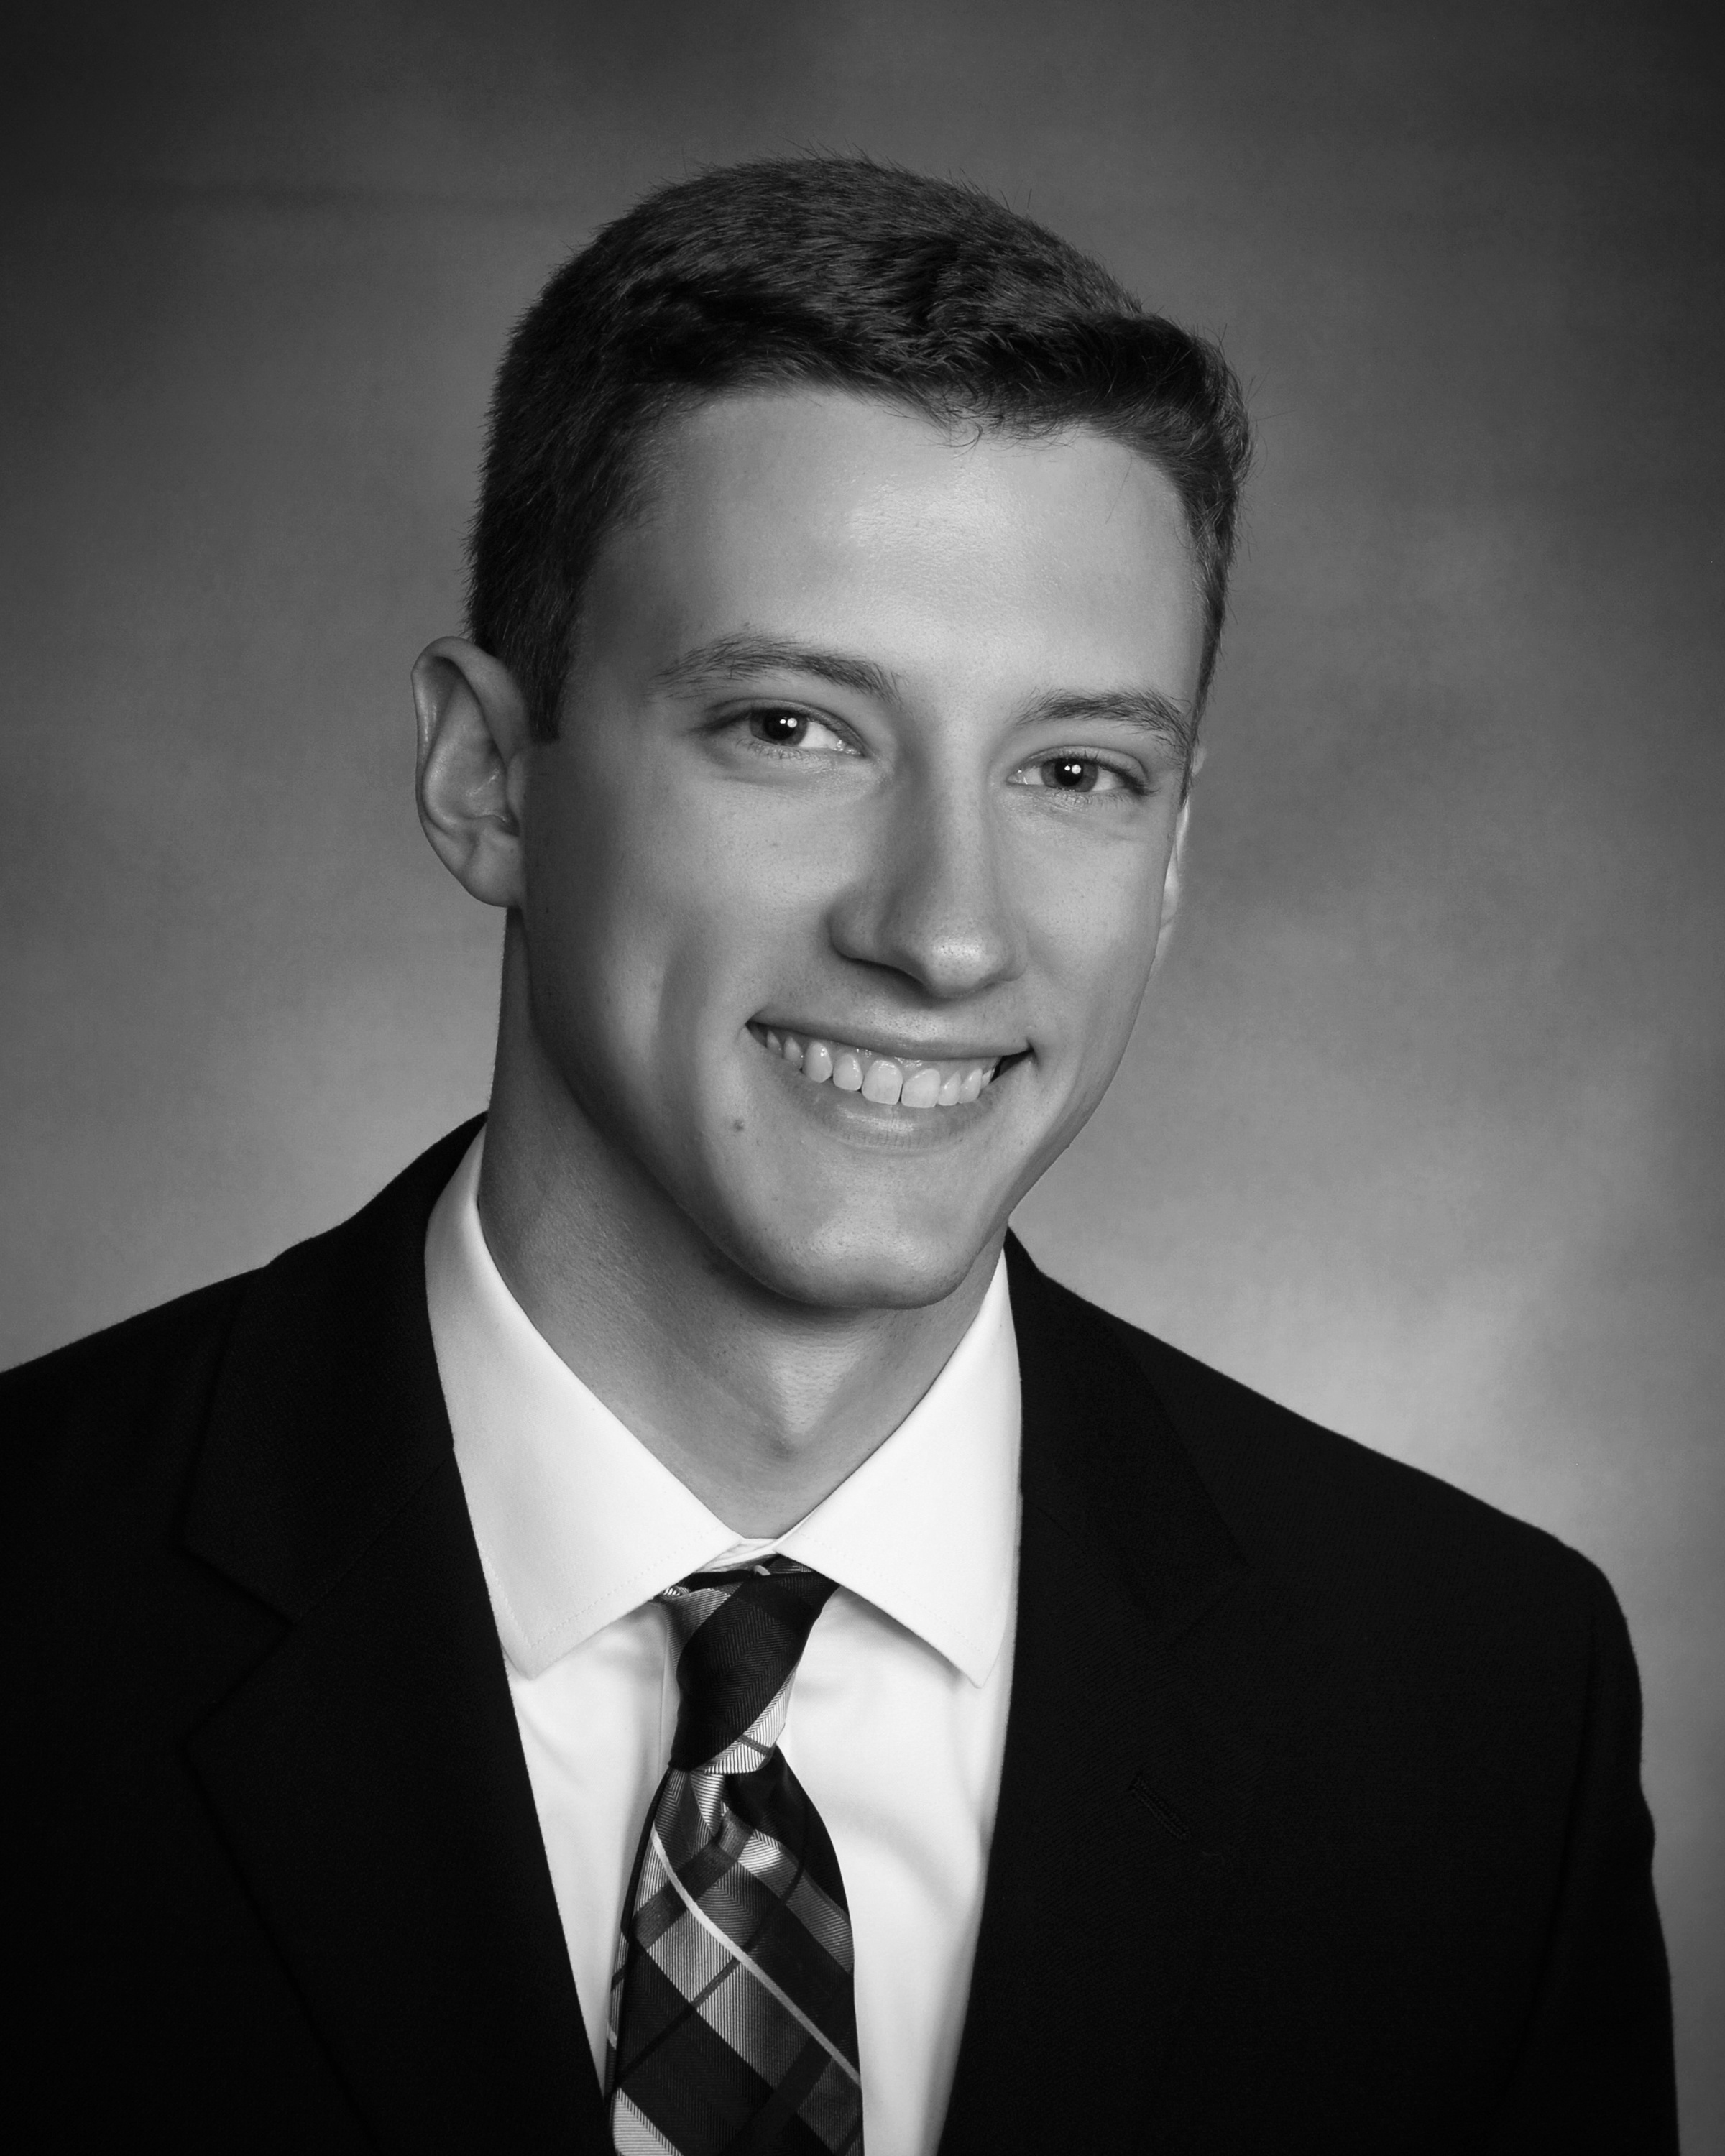
\includegraphics[width=1in,height=1.25in,clip,keepaspectratio]{sdonchez}}]
	{Stephen Donchez}
	(M'20) received his B.S. in computer engineering from Villanova University, Villanova, PA in 2020. He has remained at Villanova in pursuit of his M.S. in computer engineering, which he anticipates receiving in May of 2022.

	In the summer of 2018 he was a software engineering intern at Harris Corporation (now L3Harris Technologies, Inc.). He returned to L3Harris for the summer of 2019 as a systems engineering intern, and returned again to the same position for the summer of 2020 at their facility in Clifton, NJ, where he continues to work on a part-time basis.  He anticipates joining L3Harris's Camden facility as a Systems Engineer specializing in Cybersecurity following his Master's Program.

	His research interests include FPGAs, embedded software development, and embedded systems with a focus on System-on-a-Chip technologies and security.

	Mr. Donchez is a student member of the IEEE.
\end{IEEEbiography}


\end{document}